
In this report, we explain in detail the results and graphs that we obtained from the Mozilla build data, as well as potential questions (i.e.: \kyle{a question}). Please, take a look and tell us what you think.

Thanks in advance.

\section{\label{KYLE} Pushes not found in the Mozilla build dataset}

We discovered some interesting facts about the mozilla-central branch. In fact, until now, we always had a figure showing that the mozilla-central branch's number of builds by push varied over time. The median value would vary between 5 and 500 until release 44, then, it would stabilize around 1109, as seen in Fig~\ref{build_push_mozilla_central_alone}.

\begin{figure}[!h]
    \centering
    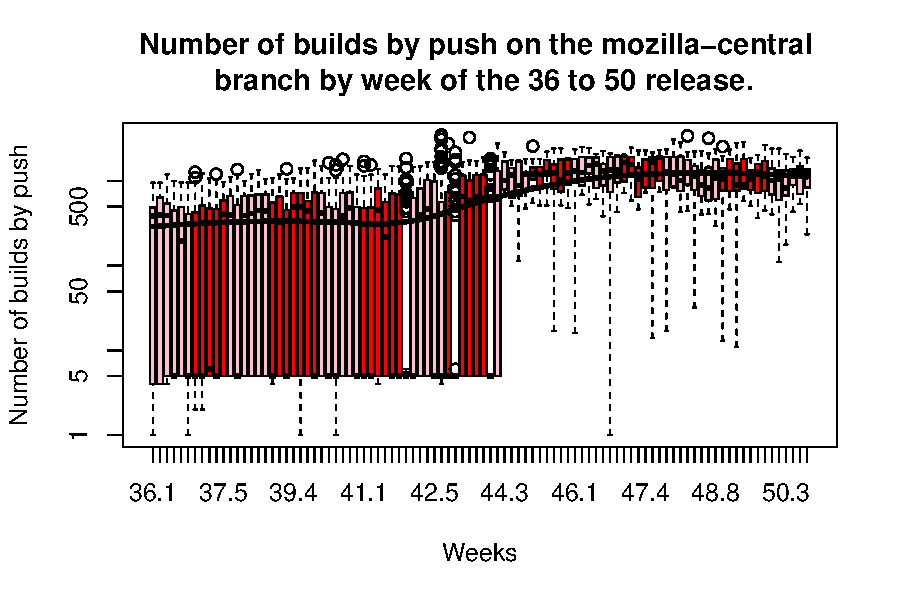
\includegraphics[width=0.45\textwidth]{img/build_push_mozilla_central.pdf}
    \caption{The number of builds by push on the mozilla-release branch varies overtime. Two states, the first one having the median varying between 5 and 500, the second one, after release 44, being around 1109.}
    \label{build_push_mozilla_central_alone}
\end{figure}

However, when we mined the mercurial mozilla-central repository and counted the number of commits for each push when associating the pushes found for the Fig~\ref{build_push_mozilla_central_alone} to those in the mercurial repository, only 57\% (1987 out of 4697) of the pushes were retrieved. That number seems odd, since, on the other branches, about 98\% of the pushes were retrieved, using the same technic.

\begin{figure}[!h]
    \centering
    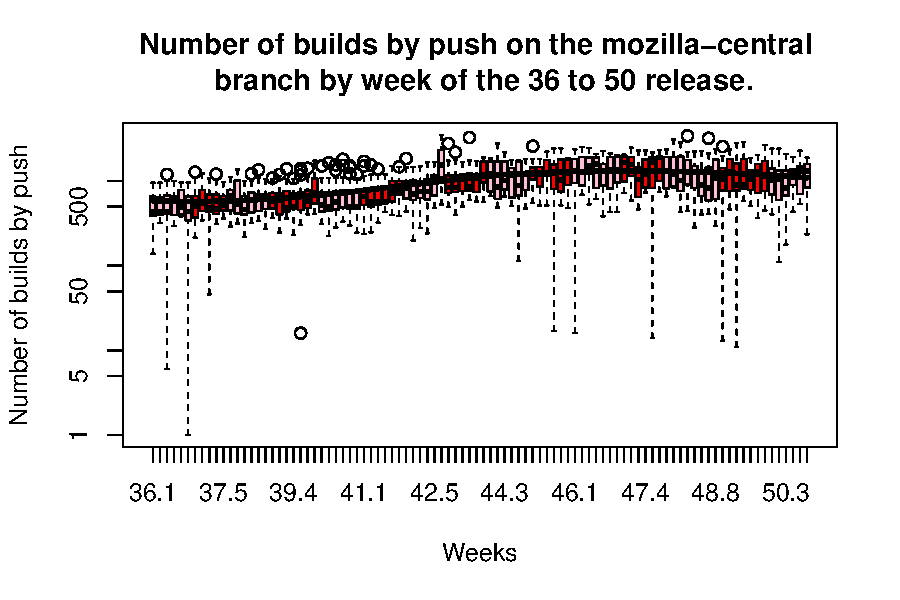
\includegraphics[width=0.45\textwidth]{img/build_push_MERCURIAL_mozilla_central.pdf}
    \caption{The number of builds by push on the mozilla-release only for the pushes \textbf{present on the mercurial repository.}}
    \label{build_push_MERCURIAL_mozilla_central_alone}
\end{figure}

To analyze this, we decided to generate the same figure as Fig~\ref{build_push_mozilla_central_alone} but only showing the pushes that were found on the mercurial repository. On the Fig~\ref{build_push_MERCURIAL_mozilla_central_alone}, we can thus see the results of that selection. The curve is here much smoother and all the pushes having 5 builds seem to have been removed.

\begin{figure}[!h]
    \centering
    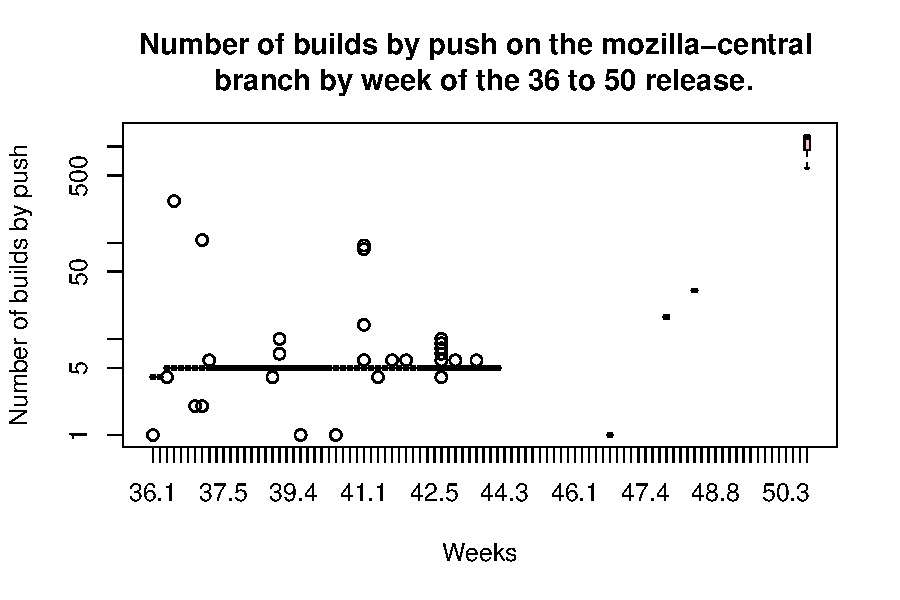
\includegraphics[width=0.45\textwidth]{img/build_push_COUNT_mozilla_central.pdf}
    \caption{The number of builds by push on the mozilla-release only for the pushes \textbf{NOT present on the mercurial repository.}}
    \label{build_push_COUNT_mozilla_central_alone}
\end{figure}

If we invert the selection, selecting only the number of builds of the pushes not found on the repository, it confirms that most of the pushes that were removed are pushes that have 5 builds (cf. Fig~\ref{build_push_COUNT_mozilla_central_alone}).

In fact, there are 1886 pushes that all run the same 5 builds : 

\begin{itemize}
    \item Firefox mozilla-central linux l10n dep  
    \item Firefox mozilla-central linux64 l10n dep 
    \item Firefox mozilla-central macosx64 l10n dep    
    \item Firefox mozilla-central win32 l10n dep    
    \item Firefox mozilla-central win64 l10n dep 
\end{itemize}


\kyle{What are those pushes that are not retrieved from the mercurial repositories ?} 

\kyle{What are the "l10n dep" builds?}

In the rest of the report, only the data regarding the pushes we found on mercurial is used. See the first part of this report for more explanations.

\newpage